\section{Agregacja krzywych dyspersji uzyskanych z zaimplementowanego solvera}
\label{sec:agregacja}

\subsection{Cel agregacji}
Podstawą opracowania każdej z przedstawionych w tej pracy metod kompensacji jest znajomość krzywych dyspersji badanego obiektu, jakim jest stalowy pręt. Stanowią one pewnego rodzaju funkcję przejścia sygnału pomiędzy jednym punktem w czasie i przestrzeni a dowolnym innym punktem. Ich znajomość stanowi więc klucz do skomensowania efektu dyspersji. W stworzonej aplikacji, dzięki zastosowaniu odpowiednich algorytmów, na podstawie odpowiednich zadanych parametrów badanego obiektu, otrzymywane są poszukiwane krzywe dyspersji. Jednak dane są one w postaci chmury punktów zapisywanych w odpowiednich plikach. Aby funkcje te nadawały się do użycia należy każdy z wygenerowanych punktów przypisać do odpowiedniej krzywej. W ten sposób uzyskane zostaną funkcje, z których każda opisywać będzie zachowanie innej postaci fali prowadzonej. Przykładowe wygenerowane krzywe dyspersji przed agregacją przedstawia rysunek 2.21

\subsection{Algorytm agregacji}
 Krzywe dyspersji wyrażają zależność liczby falowej od częstości kątowej. Jako wynik w aplikacji otrzymujemy pojedynczy wektor zawierający kolejne wartości liczby falowej oraz zestaw odpowiadających danej liczbie częstości kątowych. Pierwszym krokiem w agregacji tak zapisanych danych jest zapisanie wszystkich danych w postaci chmury punktów o dwóch współrzędnych $A=(\omega , k)$ oraz posortowanie ich rosnąco wartościami $\omega$. Liczba wygenerowanych krzywych odpowiada ilości punktów posiadających tę samą współrzędną k, ponieważ są to wartości własne równania (2.44) to dla każdej wartości k jest ich tyle samo. Każda krzywa składa się z dokładnie takiej liczby punktów jaka jest długość wektora k. Kolejnym krokiem jest przyporządkwanie pierwszych dwóch punktów do każdej z krzywych. Mając punkty uporządkowane względem $\omega$ wystarczy wybrać to o najmniejszej wartości k. Każdy z nich odpowiada kolejnemu trybowi fali. Punkty przedzielone do właściwego trybu zostają usunięte ze zbioru punktów do przydzielenia. Analogicznie postępujemy w przypadku drugiej grupy punktów. Wybieramy te o najniższej wartości k i przypisujemy do poszczególnych trybów. Agregacja kolejnych punktów musi przebiegać według innego schematu, ponieważ krzywe się wzajemnie przesinają i segregacja względem częstotliwości nie przyniesie zadowalających rezultatów. Przyjmując, że dla dowolnego modu, ostatni zagregowany punkt ma współrzędne $P_l = (\omega _l,k_l)$ z chmury punktów wybieramy zbiór potencjalnych punktów spełniających następujące warunki:
 \begin{enumerate}
 \item Wartość k potencjalnych punktów musi wynosić $k=k_p=v_k[l+1]$
 
 Gdzie $k_p$ oznacza wartość k potencjalnych punktów, $v_k$ oznazca posortowany rosnąco wektor wartości k, a $l+1$ to indeks wartości z wektora $v_k$ o jeden większy niż indeks ostatnio zagregowanego do danego trybu punktu
 \item Wartość $\omega$ potencjalnych punktów musi znajdować się w pewnym, ograniczonym otoczeniu wartości $\omega _l$
 
 Ze zbioru potencjalnych punktów, które spełniają wyżej wymienione warunki należy następnie wybrać ten, który w najepszy sposób będzie pasował do powstałego już fragmentu krzywej dyspersji. W celu wybrania najlepszego punktu obliczony zostaje kąt pomiędzy wektorami $\overrightarrow{v_1} = \overrightarrow{P_{l-1}P_l}$ oraz $\overrightarrow{v_2} = \overrightarrow{P_lP_{p_i}}$, gdzie $P_{p_i}$ oznacza i-ty potencjalny punkt ze zbioru. Sformułowanie najlepiej pasujący punkt oznacza, iż kąt pomiędzy rozważanymi wektorami, obliczany ze wzoru:
 \begin{equation}
 \alpha = \arccos\frac{\overrightarrow{v_1} \circ \overrightarrow{v_2}}{|\overrightarrow{v_1}|\cdot|\overrightarrow{v_2}|}
\end{equation}  
jest jak najbliższy zeru. Usuwając zagregowane już punkty ze zbioru punktów do przydzielenia oraz postępując w sposób analogiczny do przedstawionego, wszystkie punkty ze zbioru zostają przydzielone odpowiedniej krzywej. Wyniki agregacji zostały przedstawione na rysunku \ref{fig:krzywe_po_agregacji}
 
\begin{figure}[h]
\centering
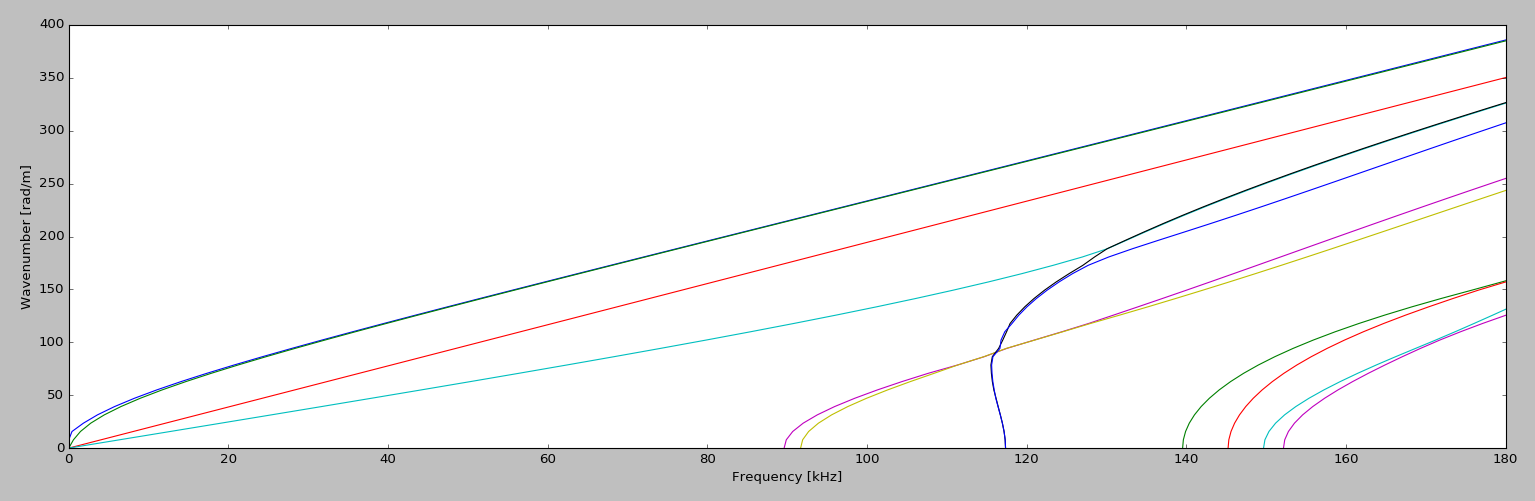
\includegraphics[width=13cm]{Zdjecia/4/zagregowane_krzywe}
\caption{Krzywe dyspersji po agregacji}
\label{fig:krzywe_po_agregacji}
\end{figure}
\end{enumerate}  

Jak łatwo zauważyć opisany algorytm w sposób efektywny agreguje chmurę punktów do odpowiednich krzywych. Uporządkowoane w ten sposób punkty zostały wykorzystane do opracowania trzech metod kompensacji, które zostały opisane w kolejnych sekcjach tego rozdziału.




